%%%design overview over libpninx

The aim of \pninx\ is to provide an easy to use but yet powerful interface
to write Nexus files from C++. Although the Nexus group already provides 
an binding of their Nexus API (NAPI) for C++, this is not much more than a 
thin wrapper around the C library. Thus the native C++ API suffers from 
a whole bunch of features that a C++ programmer would expect from an API. 
\pninx\ is an approach to overcome the limitations of the native C++ API 
and provide you with all the object oriented features that C++ exposes.

In this chapter the general design of the library will be discussed. 
Though this section is usualy for developers only, users of the library 
are highly encouraged to read this chapter as it provides a lot of useful 
information about the philosophy behind certain objects. In particular 
section~\ref{section:nxfield_design} should be read by all users of \pninx. 

\section{Classes and implementation}\label{section:classes_implementation}

%%%----------------------------------------------------------------------------
\begin{figure}[tb]
\centering
\begin{minipage}[c]{0.5\linewidth}
\centering
\resizebox{\linewidth}{!}{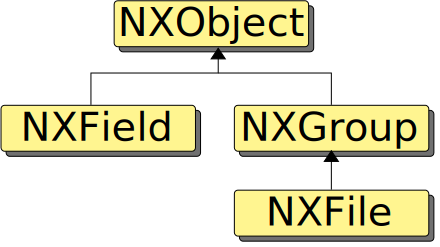
\includegraphics{pics/class_inheritance.pdf}}
\end{minipage}
\hfill
\begin{minipage}[c]{0.49\linewidth}
\caption{{\small\label{fig:class_inheritance}
Inheritance relations between the major objects provided by \pninx.
\nxobject\ is the root of the class tree but will hardly be used. 
The class important to a developer are the three classes derived from 
\nxobject: \nxfield, \nxgroup, and \nxfile.
}}
\end{minipage}
\end{figure}
%%%----------------------------------------------------------------------------
In order to remain simple to use \pninx\ exposes only four classes to the 
user where only three are needed in real world applications in order to 
read and write data. 
Figure~\ref{fig:class_inheritance} shows the inheritance tree of the 
exposed classes. The top-level object is \nxobject. This class 
collates all methods common to each object in the tree. However, you hardly 
ever use \nxobject\ in your code. The only classes relevant for users
are
\begin{description}
\item[\nxgroup] the standard container to hold all kinds of objects
\item[\nxfield] the data holding objects
\item[\nxfile] object representing a data file.
\end{description}
\nxfile is a descandent of \nxgroup\ as can be seen in
Fig.~\ref{fig:class_inheritance}. Thus it posses all the functionality that 
\nxgroup\ has aside from those methods necessary for file handling. 
\pninx\ uses HDF5 to write data to disk. However, you do not have to know 
anything about HDF5. No low level HDF5 calls are necessary. Everything is 
masked by the three objects mentioned above. 
In order to do so a Bridge pattern~\cite{book:gof} was used for the
implementation. The idea was to separate the interface provided to the user from the 
concrete interface used to communicate with the HDF5 library. 
This allows us to change the HDF5 backend completely without changing 
user code using the library (maybe recompilation is needed - but this is not as
bad as changing code). This gives us much more freedom in maintaining \pninx.
The bridge pattern is not implemented as shown in \cite{book:gof} but rather 
by using a template approach as shown  in \cite{book:alexandrescu}.
Hence the code remains free of pointers which makes it much more readable. 
Furthermore it should be mentioned that the \pninx\ heavily relies on features 
provided by the C++11 standard. Thus, an actuall compiler is required to 
build the library.
 

\section{A closer view on \nxfield}\label{section:nxfield_design}
\nxfield\ is most probably the most important object in the \pninx-universe. 
Objects of type \nxfield\ are used to read and write data to the file. 
This section is thus not only important for library developers but also 
for those who simply want to use \pninx. 
From the point of C++, \nxfield\ can be considered a container like 
{\tt std::vector<>} or {\tt std::list<>}.
There are basically two kinds of objects that can be stored in this container
\begin{enumerate}
  \item numerical data
  \item strings
  \item and binary uninterpreted data.
\end{enumerate}
\nxfield\ is treated differently depending on the type of data that should 
be stored in the container.
When an \nxfield\ object is newly instantiated it represents an empty container. 
Writing data to disk means nothing else than appending data to the container. 
Reading data is the inverse operation - fetching data from the container. 
The size (number of elements) of the container is limited by the amount of 
free space on the storage device on which the file is writen.
\nxfield\ mimics up to some point the behavior of the container objects
provided by the C++ standard library. So you will find methods like 
{\tt get()}, {\tt insert()}, {\tt append()} and so on. 
Now, depending on the type of data that should be stored  the container 
behaves slightly different. 
Numerical data can be either a single number or a multidimensional array of 
data that is stored in each container entry. 
For binary data only one element of data can be stored.


 

